\section{Deep Gated Network}\label{sec:pathgate}
\FloatBarrier
\begin{table}[h]
\begin{minipage}{0.5\columnwidth}
\resizebox{\columnwidth}{!}{
\begin{tabular}{|l|l|}\hline
\multicolumn{2}{|c|}{Deep Gated Network: $\N(\Theta_t;\G_t)$}\\\hline 
Input layer & $z_{x,\Theta_t}(0)=x$ \\\hline
Pre-activation & $q_{x,\Theta_t}(l)={\Theta_t(l)}^\top z_{x,\Theta_t}(l-1)$\\\hline
Layer output & $z_{x,\Theta_t}(l)=q_{x,\Theta_t}(l)\odot G_{x,t}(l)$ \\\hline
Final output & $\hat{y}_t(x)={\Theta_t(d)}^\top z_{x,\Theta_t}(d-1)$\\\hline
Gating Values& $\begin{aligned}\G_t\stackrel{def}=\{G_{x_{s},t}(l,i), \forall s\in[n],\\l\in[d-1],i\in[w]\}\end{aligned}$\\\hline
\end{tabular}
}
\end{minipage}
\begin{minipage}{0.5\columnwidth}
\resizebox{\columnwidth}{!}{
\begin{tabular}{|c|c|}\hline
Gating Network: $\G(\Tg_t,\beta)$\\\hline
$z_{x,\Tg_t}(0)=x$  \\\hline
$q_{x,\Tg_t}(l)={\Tg_t(l)}^\top z_{x,\Tg_t}(l-1)$ \\\hline
$z_{x,\Tg_t}(l)=q_{x,\Tg_t}(l)\odot G_{x,\Tg_t}(l)$ \\\hline
{$\begin{aligned}\beta >0: G_{x,\Tg_t}(l,i)&=\frac{1+\epsilon}{1+\exp(-\beta q_{x,\Tg_t}(l,i))} \\ \beta=\infty: G_{x,\Tg_t}(l,i)&=\mathbbm{1}_{\{q_{x,\Tg_t}(l,i)>0\}}\end{aligned}$}\\\hline 
\end{tabular}
}
\end{minipage}
\caption{Here $\Theta(l,i,j)$ denotes the weight connecting node $i$ of layer $l-1$ to node $j$ of layer $l$, and $\odot$ stands for the \emph{Hadamard} product. The left table shows a DGN, and the right table shows a gating network. }
\label{tb:dgn}
\end{table}
We denote the dataset is given by $(x_s,y_s)_{s=1}^n$, the data matrix is given by $x=(x_s,s\in[n])\in\R^{d_{in}\times n}$, and $y_s\in\R$ in the case of regression and $y_s\in[C]$ in the case of $C$-class classification. Further, let $y=(y_s,s\in[n])$ be the vector of labels. We consider fully connected deep gated networks with $d$ layers (i.e., depth $=d$), and $w$ hidden units per layer (i.e., width $=w$). In \Cref{tb:dgn}, $q(l),z(l)$ and $G(l)$ are $w$-dimensional quantities, where $G(l)$ are the gating values.  At at time $t$, by specifying the gating values for all the $n$ input examples as $\G_t\stackrel{def}=\{G_{x_{s},t}(l,i), \forall s\in[n],l\in[d-1],i\in[w]\}$, we can recover the outputs $\hat{y}_t(x_s)\in \R$ for all the inputs $\{x_s\}_{s=1}^n$ in the dataset.  A DGN is denoted by $\N(\Theta_t;\G_t)$, i.e., the weights and the gating values are decoupled, and need to be specified to obtain a complete description. The gating values can also be obtained from a different gating network, parameterised by $\Tg\inrdnet$: we denote the gating values by $\G(\Tg_t,\beta)$. We also consider soft-gating, which uses a sigmoidal function: desirable feature here is that the gating values are differentiable with respect to the underlying parameter. Following the notational conventions, a DNN with ReLU activations is denoted by $\N(\Theta_t;\G(\Theta_t,\infty))$.\begin{comment}
The DGN framework allows us the flexibility to study a host of deep networks with different gating mechanisms. The gates can be fixed (i.e., $\G_t=\G_0,\forall t\geq 0$) or learnable, i.e., $\G_t$ changes during training. The gates can be parameterised explicitly with $\Tg\neq \Theta$, or implicitly with $\Tg=\Theta$, or unparameterised. Further, the gating can be hard taking values in $\{0,1\}$ or soft taking values in $(0,1+\epsilon)$.
\end{comment}
\begin{figure}
%\begin{minipage}{0.78\columnwidth}
\resizebox{\columnwidth}{!}{
\begin{tabular}{ccc}
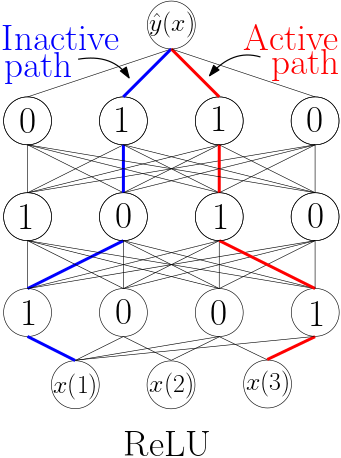
\includegraphics[scale=0.5]{figs/nn.png}
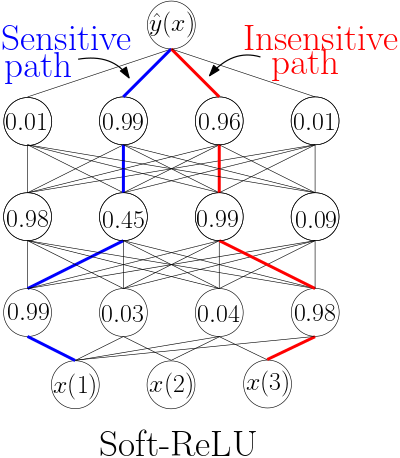
\includegraphics[scale=0.5]{figs/nnsoft.png}
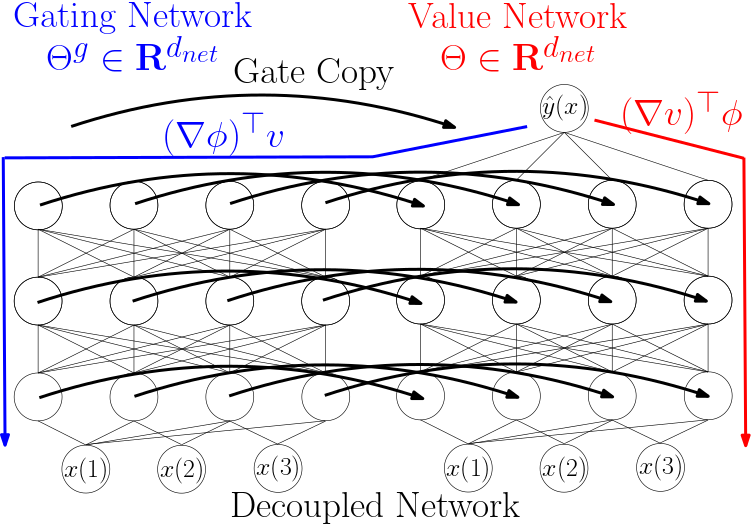
\includegraphics[scale=0.5]{figs/nntwin.png}
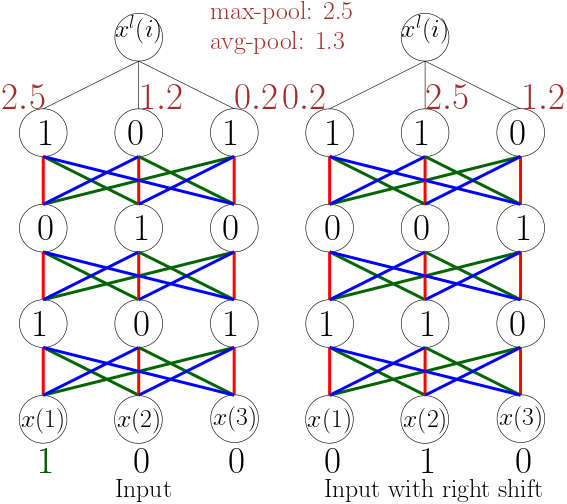
\includegraphics[scale=0.5]{figs/nnconv.png}
%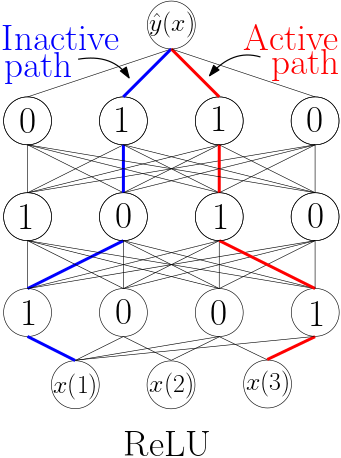
\includegraphics[scale=0.5]{figs/nn.png}
%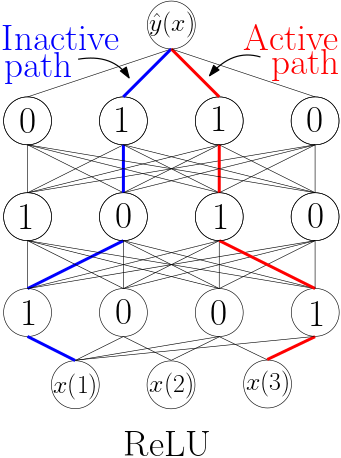
\includegraphics[scale=0.5]{figs/nn.png}
\end{tabular}
}
%\end{minipage}
%\begin{minipage}{0.18\columnwidth}
%\resizebox{\columnwidth}{!}{
%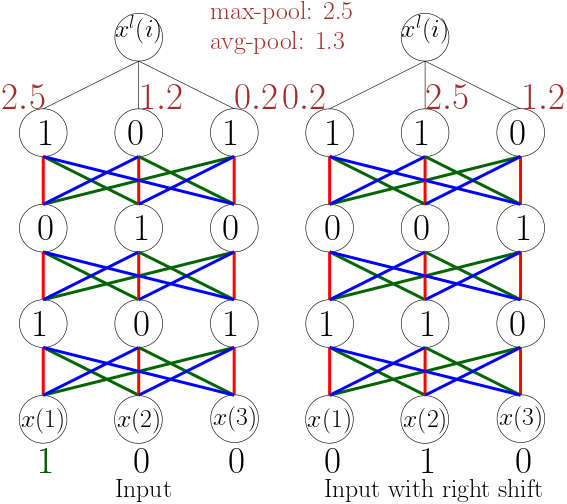
\includegraphics[scale=0.5]{figs/nnconv.png}
%}
%\end{minipage}

\end{figure}
